% =====================================================================
% TEMPLATE DỊCH SÁCH SANG TIẾNG VIỆT
% Biên dịch bằng XeLaTeX (KHÔNG dùng pdflatex, sẽ lỗi font/dấu)
% =====================================================================
\documentclass[12pt,a4paper, openany]{book}

% ---------------------------------------------------------------------
% 1. FONT & NGÔN NGỮ TIẾNG VIỆT
% ---------------------------------------------------------------------
\usepackage{fontspec}
\usepackage{polyglossia}
\setmainlanguage{vietnamese}

% Noto Serif/Sans hỗ trợ đầy đủ dấu tiếng Việt trên Overleaf.
% Tự động fallback sang Times New Roman / Arial / Consolas khi biên dịch trên máy cục bộ chưa có Noto:
\IfFontExistsTF{Noto Serif}{
  \setmainfont{Noto Serif}[Ligatures=TeX]
  \setsansfont{Noto Sans}
  \setmonofont{Noto Sans Mono}
}{
  \setmainfont{Times New Roman}[Ligatures=TeX]
  \setsansfont{Arial}
  \setmonofont{Consolas}
}

% ---------------------------------------------------------------------
% 2. KHỔ TRANG & DÃN DÒNG
% ---------------------------------------------------------------------
\usepackage[a4paper,top=2.5cm,bottom=2.5cm,left=3cm,right=2cm,headheight=16pt]{geometry}
\usepackage{setspace}
\onehalfspacing

% ---------------------------------------------------------------------
% 3. ĐỊNH DẠNG TIÊU ĐỀ CHƯƠNG
% ---------------------------------------------------------------------
\usepackage{titlesec}
\titleformat{\chapter}[display]
  {\normalfont\huge\bfseries}
  {\chaptertitlename\ \thechapter}
  {20pt}{\Huge}
\titlespacing*{\chapter}{0pt}{0pt}{40pt}

% ---------------------------------------------------------------------
% 4. ĐẦU TRANG / CHÂN TRANG
% ---------------------------------------------------------------------
\usepackage{fancyhdr}
\pagestyle{fancy}
\fancyhf{}
\fancyhead[LE,RO]{\thepage}
\fancyhead[RE]{\nouppercase{\leftmark}}
\fancyhead[LO]{\nouppercase{\rightmark}}
\renewcommand{\headrulewidth}{0.4pt}

% ---------------------------------------------------------------------
% 5. ẢNH, TOÁN, MÀU, LIÊN KẾT, TRÍCH DẪN
% ---------------------------------------------------------------------
\usepackage{amsmath}
\usepackage{amssymb}
\usepackage{graphicx}
\usepackage[dvipsnames]{xcolor}
\usepackage{csquotes}
\usepackage{placeins}
\usepackage[hidelinks]{hyperref}
\hypersetup{
    pdftitle={Tên sách (bản dịch)},
    pdfauthor={Tên dịch giả},
}

\begin{document}

% =====================================================================
% BÌA SÁCH
% =====================================================================
\begin{titlepage}
    \centering
    \vspace*{2cm}

    {\Large \textsc{MATTHEW O. WARD, GEORGES GRINSTEIN, \\ DANIEL KEIM}}\\[0.6cm]
    \rule{0.8\textwidth}{0.4pt}\\[0.5cm]

    {\huge \bfseries TRỰC QUAN HÓA DỮ LIỆU TƯƠNG TÁC TỪ NỀN TẢNG, KĨ THUẬT ĐẾN ỨNG DỤNG}\\[0.4cm]
    {\Large \textit{Nguyên tác: \textit{Interactive Data Visualization - Foundations, Techniques, and Applications}}}\\[0.5cm]
    \rule{0.8\textwidth}{0.4pt}\\[2cm]

    % Nếu có ảnh bìa gốc, bỏ % dòng dưới và đổi tên file ảnh:
    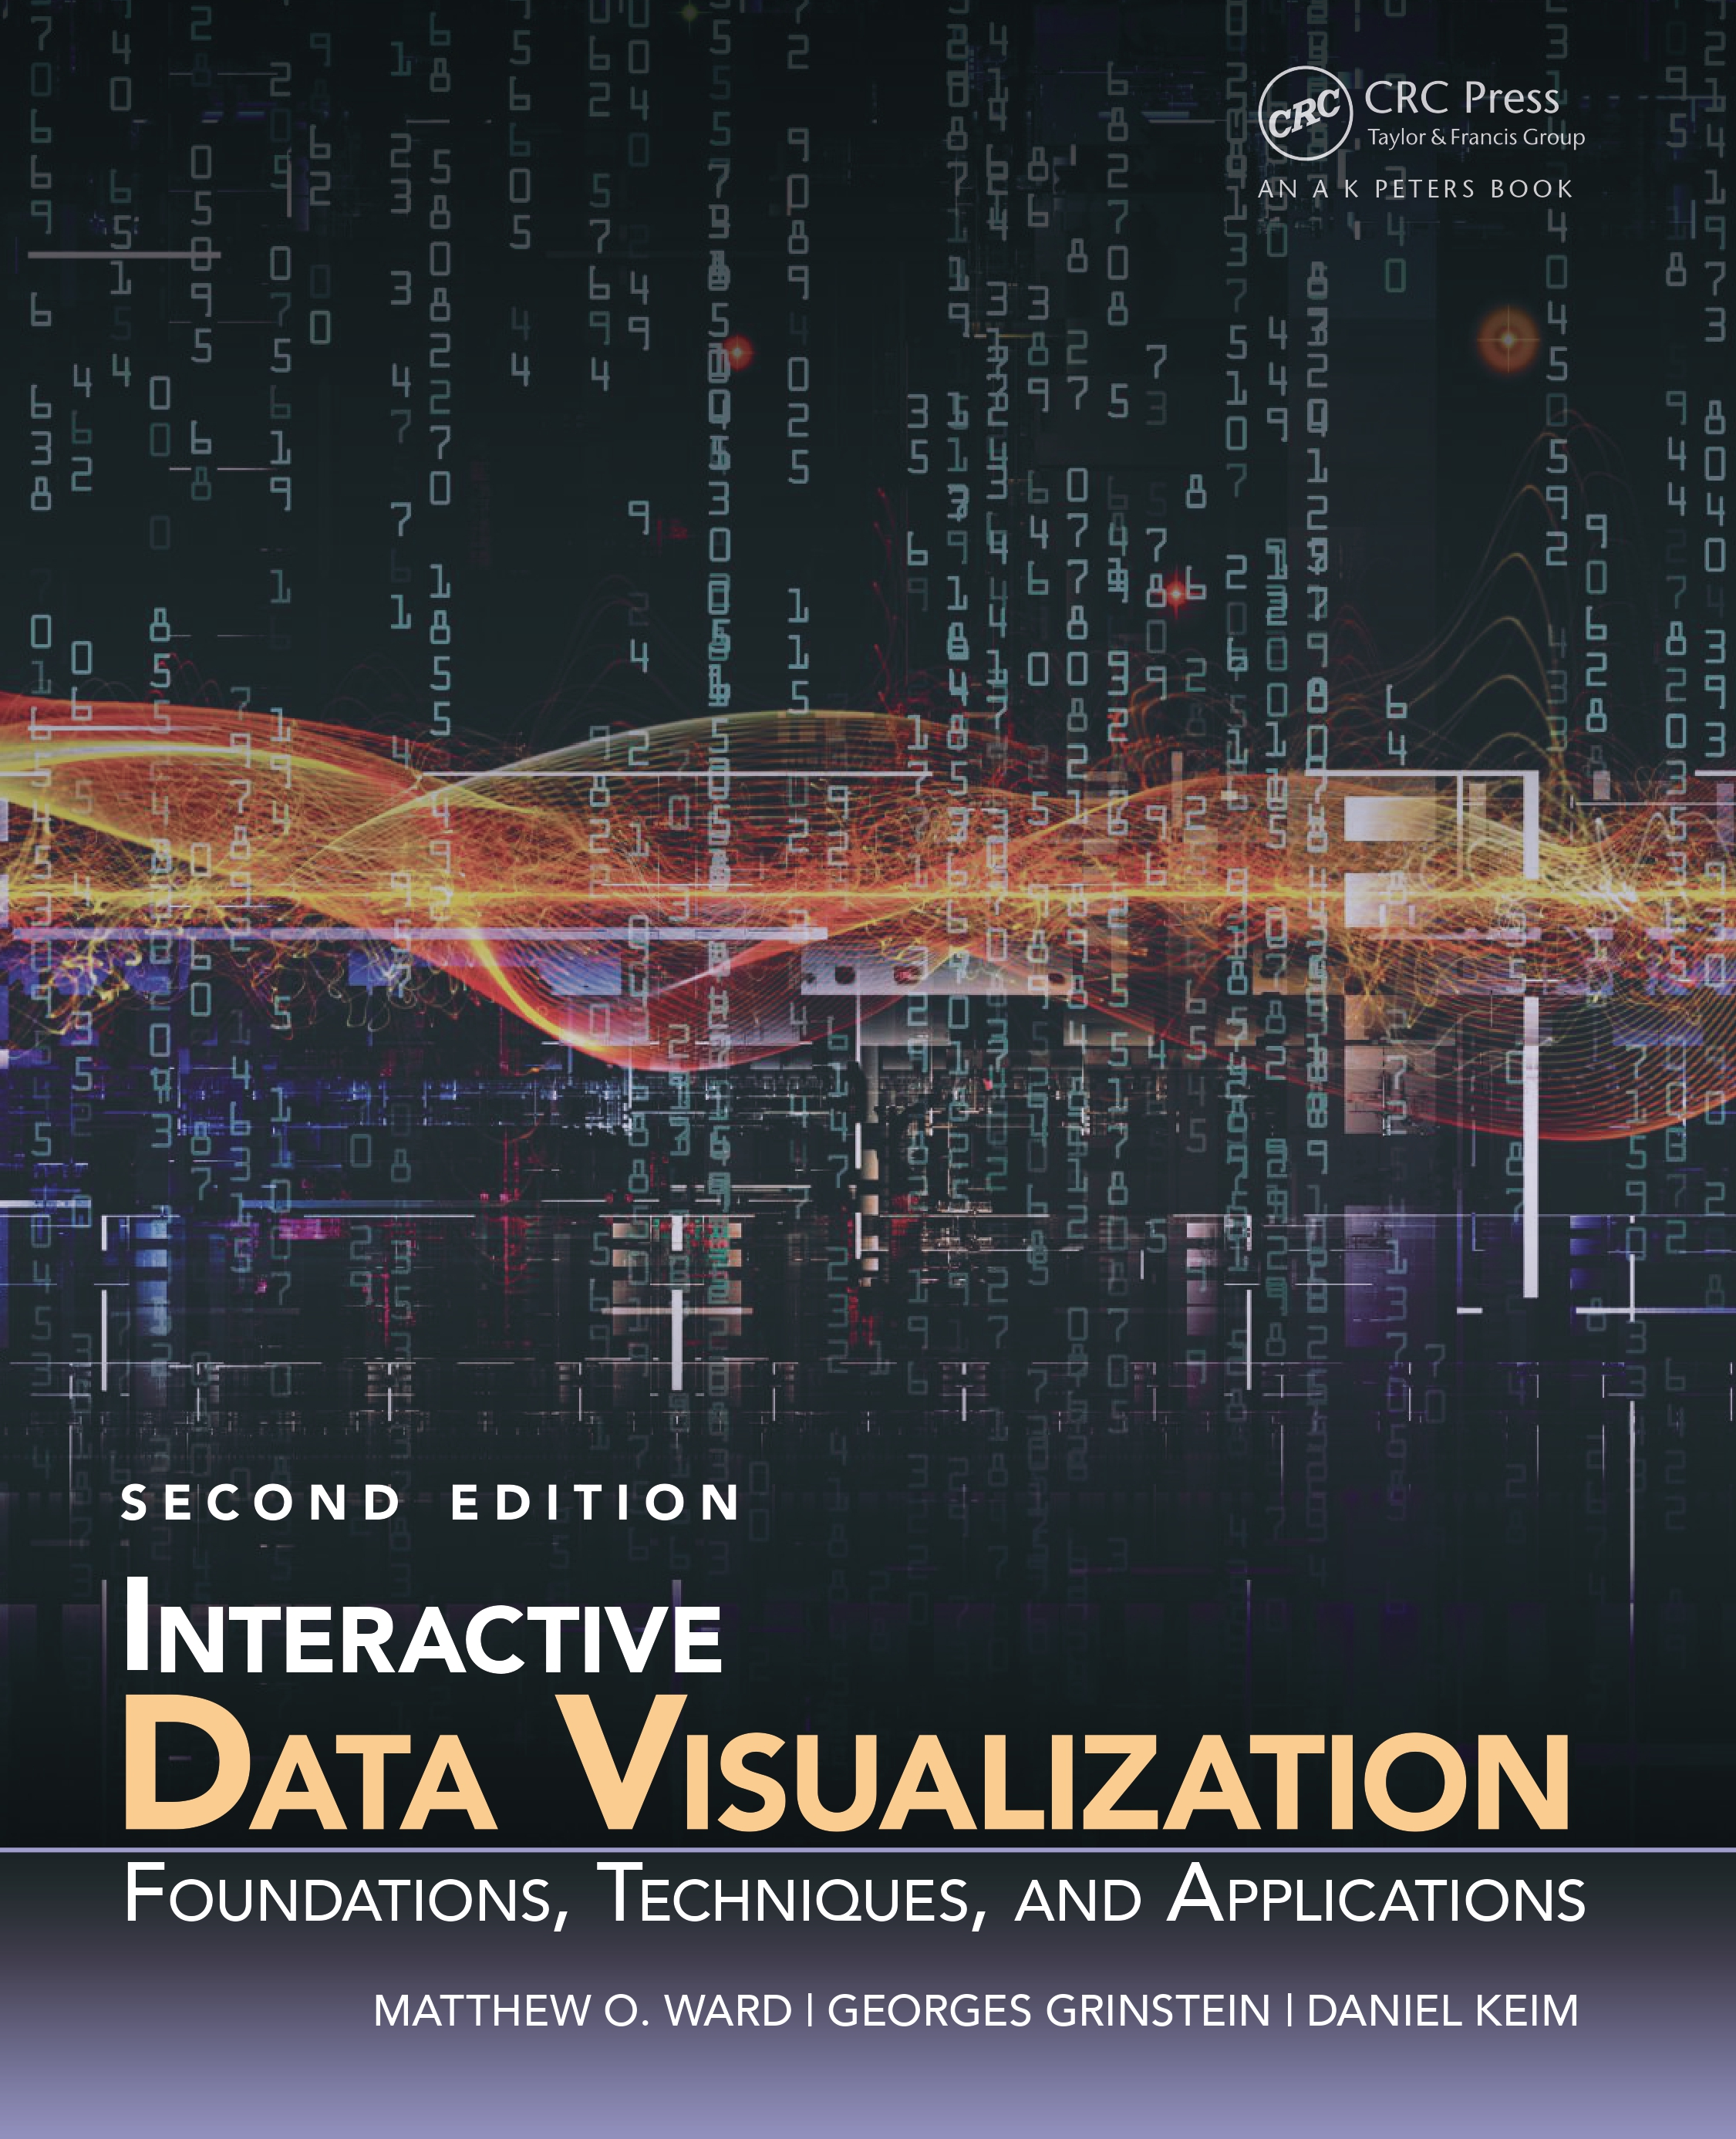
\includegraphics[width=0.35\textwidth]{img/cover-image.jpg}\\[0.5cm]

    \vfill

    {\large\textbf{Chương 9. Kỹ thuật trực quan hóa cho Cây, Đồ thị và Mạng}}\\[0.3cm]
    {\normalsize Nguyễn Việt Phúc, Dương Quang Huy, Nguyễn Khắc Huy}\\[1cm]

    {\large \today}
\end{titlepage}

% ---------------------------------------------------------------------
% TRANG PHÂN CÔNG
% ---------------------------------------------------------------------
\newpage
\thispagestyle{empty}
\vspace*{4cm}
\noindent
\begin{center}
    {\Large\textbf{PHÂN CÔNG CÔNG VIỆC}}
\end{center}

\vspace{1.5cm}

\renewcommand{\arraystretch}{1.5}
\begin{table}[h]
\centering
\begin{tabular}{|p{4cm}|p{2.5cm}|p{7.5cm}|}
\hline
 Nguyễn Khắc Huy & 23001525 & Phần 9.1. Biểu diễn cấu trúc Phân cấp \\
\hline
 Nguyễn Việt Phúc & 23001547 & Phần 9.2. Biểu diễn Đồ thị, Mạng tùy ý\\
\hline
 Dương Quang Huy & 23001524 & Phần 9.3. Các vấn đề khác \newline Phần 9.4. Tài liệu tham khảo\\
\hline
\end{tabular}
\end{table}

% =====================================================================
% MỤC LỤC
% =====================================================================
\frontmatter
\tableofcontents

% ---------------------------------------------------------------------
% LỜI NGƯỜI DỊCH (không đánh số chương)
% ---------------------------------------------------------------------
\chapter*{Lời người dịch}
\addcontentsline{toc}{chapter}{Lời người dịch}

\textit{Interactive Data Visualization: Foundations, Techniques, and Applications} của Matthew O. Ward, Georges Grinstein và Daniel Keim là một trong những giáo trình nền tảng của lĩnh vực trực quan hóa dữ liệu. Điểm khiến cuốn sách này khác với phần lớn tài liệu cùng chủ đề là nó không dừng ở việc giới thiệu hình thức bề ngoài của các biểu đồ, mà đi thẳng vào thuật toán sinh ra chúng: mỗi kỹ thuật đều được trình bày kèm mã giả, kèm những ràng buộc thiết kế và những đánh đổi mà người cài đặt buộc phải cân nhắc.

Chúng tôi chọn dịch Chương 9 --- \textit{Visualization Techniques for Trees, Graphs, and Networks} --- vì hai lý do. Thứ nhất, cây và đồ thị là hai cấu trúc quan hệ phổ biến nhất trong thực tế, từ sơ đồ tổ chức, cây phân loại sản phẩm cho đến mạng xã hội và mạng lưới thương mại giữa các quốc gia; nắm được cách trực quan hóa chúng là nắm được một công cụ dùng lại được ở rất nhiều bài toán. Thứ hai, đây cũng chính là họ kỹ thuật mà nhóm sử dụng cho đồ án cuối kỳ của môn học, nên việc dịch chương này vừa là bài tập ngôn ngữ, vừa là bước đọc tài liệu chuẩn bị cho phần thực hành phía sau.

Trong quá trình chuyển ngữ, chúng tôi đặt tính chính xác về mặt kỹ thuật lên trước sự mượt mà của câu văn. Ở những chỗ hai yêu cầu này xung đột, chúng tôi chọn cách diễn đạt sát với ý đồ của tác giả, kể cả khi câu tiếng Việt vì thế mà dài hơn. Một số quy ước cụ thể đã được thống nhất giữa ba người dịch:

\begin{itemize}
    \item \textbf{Thuật ngữ đã thành tên riêng quốc tế được giữ nguyên.} Các tên như \textit{treemap}, \textit{sunburst}, \textit{node-link}, \textit{force-directed}, \textit{cone tree}, \textit{roll-up}, \textit{drill-down} đều được giữ ở dạng gốc. Đây là những từ mà người đọc sẽ gặp lại nguyên văn trong tài liệu chuyên ngành, thư viện phần mềm và các bài báo sau này; dịch chúng ra tiếng Việt sẽ tạo thêm một lớp trung gian không cần thiết. Riêng từ \textit{node}, chúng tôi giữ nguyên thay vì dịch thành ``nút'' để tránh nhầm lẫn với nghĩa thông thường của từ này trong tiếng Việt, trong khi \textit{edge} được dịch thống nhất là ``cạnh''.

    \item \textbf{Mã giả được giữ nguyên tiếng Anh.} Các khối mã giả trong sách là mã lệnh chứ không phải văn xuôi. Dịch tên biến và từ khóa sang tiếng Việt sẽ khiến chúng không còn đối chiếu được với bản gốc và không còn dùng được khi cài đặt. Chỉ phần chú thích hình bên dưới mỗi khối mã được dịch.

    \item \textbf{Số hiệu tài liệu tham khảo được giữ theo bản gốc.} Các ký hiệu dạng [206], [341], [393]\ldots trong bản dịch tương ứng với danh mục tham khảo ở cuối sách gốc. Chúng tôi không đánh số lại để người đọc có thể tra cứu trực tiếp về nguyên tác.

    \item \textbf{Hình minh họa được trích từ bản gốc.} Các hình được giữ nguyên nội dung và số hiệu; chỉ phần chú thích được dịch.

    \item \textbf{Các chú thích chân trang là phần bổ sung của người dịch,} không có trong nguyên tác. Chúng tôi thêm vào ở những chỗ mà bản gốc nêu kết luận nhưng lược bỏ lập luận dẫn tới kết luận đó, nhằm giúp người đọc chưa có nền tảng về đồ thị theo được mạch trình bày.
\end{itemize}

Chương 9 được chia cho ba người: Nguyễn Khắc Huy dịch Phần 9.1 (Biểu diễn cấu trúc phân cấp), Nguyễn Việt Phúc dịch Phần 9.2 (Biểu diễn đồ thị, mạng tùy ý), Dương Quang Huy dịch Phần 9.3 (Các vấn đề khác) và Phần 9.4 (Đọc thêm). Dù mỗi người phụ trách một phần riêng, bảng thuật ngữ và các quy ước trình bày được thống nhất chung từ đầu và toàn bộ bản dịch đã được cả ba cùng rà soát chéo để bảo đảm cách dùng từ nhất quán xuyên suốt.

Chúng tôi ý thức rằng đây là bản dịch của những người còn đang học, thực hiện trong khuôn khổ một bài tập môn học chứ không phải một ấn phẩm chuyên nghiệp. Những thiếu sót về cách diễn đạt và về thuật ngữ là khó tránh khỏi. Chúng tôi rất mong nhận được góp ý từ thầy cô và các bạn đọc để bản dịch được hoàn thiện hơn.

\vspace{0.8cm}
\begin{flushright}
    \textit{Nhóm dịch}
\end{flushright}

% =====================================================================
% NỘI DUNG CHÍNH
% =====================================================================
\mainmatter

\chapter*{Phần 9.1. \newline Biểu diễn cấu trúc Phân cấp}
\addcontentsline{toc}{chapter}{Phần 9.1. Biểu diễn cấu trúc Phân cấp}
\markboth{Phần 9.1. Biểu diễn cấu trúc Phân cấp}{}

Cây, hay cấu trúc phân cấp (sách sẽ dùng hai thuật ngữ này thay thế cho nhau), là một trong những cấu trúc phổ biến nhất để lưu giữ thông tin quan hệ. Chính vì vậy, rất nhiều kỹ thuật trực quan hóa đã được phát triển để hiển thị loại thông tin này. Ta có thể chia các kỹ thuật đó thành hai lớp thuật toán: lấp đầy không gian và không lấp đầy không gian. Phần còn lại của mục này sẽ trình bày chi tiết cách cài đặt các thuật toán trực quan hóa loại dữ liệu này.

\section*{9.1.1. Các phương pháp lấp đầy không gian}
\addcontentsline{toc}{section}{Phần 9.1.1. Các phương pháp lấp đầy không gian}

Đúng như tên gọi, các kỹ thuật lấp đầy không gian tận dụng tối đa không gian hiển thị. Điều này đạt được bằng cách dùng phép đặt kề để hàm ý quan hệ, thay vì biểu đạt quan hệ bằng những cạnh nối các đối tượng dữ liệu như ở các cách tiếp cận khác. Hai hướng tiếp cận phổ biến nhất để sinh ra các cấu trúc phân cấp lấp đầy không gian là bố cục chữ nhật và bố cục xuyên tâm.

\subsubsection{Bố cục chữ nhật}

Treemap [206] cùng vô số biến thể của nó là một cách biểu diễn thay thế cho biểu đồ Venn, và là dạng phổ biến nhất của bố cục chữ nhật lấp đầy không gian. Trong treemap cơ bản, một hình chữ nhật được chia đệ quy thành các lát, luân phiên cắt theo phương ngang và phương dọc, dựa trên số lượng phần tử của các cây con ở tầng đang xét. Mã giả của quá trình này được cho ở Hình \ref{fig:treemap_code}, và một ví dụ được trình bày ở Hình \ref{fig:treemap}.

Như đã đề cập, nhiều biến thể của treemap đã được đề xuất và phát triển kể từ khi kỹ thuật này ra đời, trong đó có treemap vuông hóa [51] (tối ưu hóa việc phân chia sao cho tỉ lệ khung hình của mỗi ô gần với hình vuông nhất có thể)\footnote{Thuật toán mặc định chia lát cắt luân phiên theo một chiều cố định cho mỗi tầng, điều này tạo ra các ô rất dài và hẹp khi có nhiều node lá, gây khó khăn cho việc tương tác chọn lựa bằng chuột, ước lượng diện tích bằng mắt và hiển thị nhãn văn bản.} và treemap lồng nhau [206] (nhằm làm nổi bật cấu trúc phân cấp).

\begin{figure}[htbp]
\centering
\par\noindent\rule{0.95\linewidth}{0.5pt}\par\vspace{4pt}
\begin{minipage}{0.9\linewidth}
\singlespacing
\footnotesize
\begin{verbatim}
Start: Main Program
  Width = width of rectangle
  Height = height of rectangle
  Node = root node of the tree
  Origin = position of rectangle, e.g., [0,0]
  Orientation = direction of cuts, alternating
                between horizontal and vertical
  Treemap(Node, Orientation, Origin, Width, Height)
End: Main Program

Treemap(node n, orientation o, position orig, hsize w, vsize h)
  if n is a terminal node (i.e., it has no children)
    draw_rectangle(orig, w, h)
    return
  for each child of n (child_i), get number of terminal nodes in subtree
  sum up number of terminal nodes
  compute percentage of terminal nodes in n from each subtree (percent_i)
  if orientation is horizontal
    for each subtree
      compute offset of origin based on origin and width (offset_i)
      treemap(child_i, vertical, orig + offset_i, w * percent_i, h)
  else
    for each subtree
      compute offset of origin based on origin and height (offset_i)
      treemap(child_i, horizontal, orig + offset_i, w, h * percent_i)
End: Treemap
\end{verbatim}
\end{minipage}
\par\vspace{6pt}\noindent\rule{0.95\linewidth}{0.5pt}\par
\caption{Mã giả vẽ một cấu trúc phân cấp bằng treemap.}
\label{fig:treemap_code}
\end{figure}

\begin{figure}[htbp]
    \centering
    \begin{minipage}{0.48\linewidth}
        \centering
        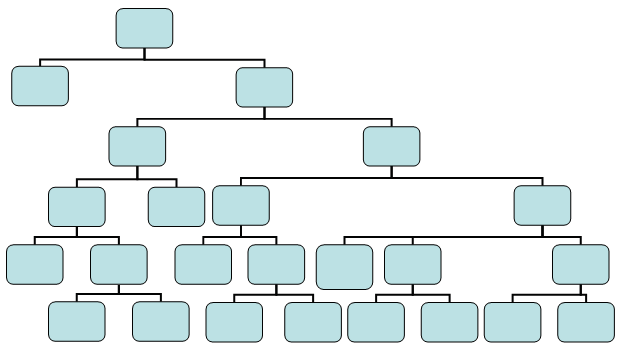
\includegraphics[width=0.85\linewidth]{img/fig9-2a-hierarchy.png}
        \par\vspace{4pt}{\small (a) Cấu trúc phân cấp mẫu}
    \end{minipage}\hfill
    \begin{minipage}{0.48\linewidth}
        \centering
        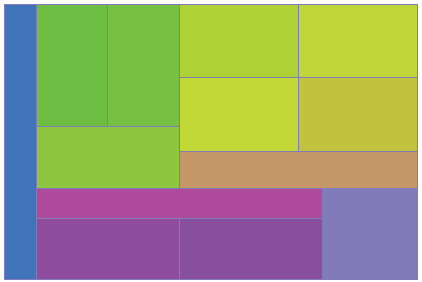
\includegraphics[width=0.85\linewidth]{img/fig9-2b-treemap.png}
        \par\vspace{4pt}{\small (b) Treemap tương ứng}
    \end{minipage}
    \caption{Một cấu trúc phân cấp mẫu và biểu đồ treemap tương ứng.}
    \label{fig:treemap}
\end{figure}

\FloatBarrier
\subsubsection{Bố cục xuyên tâm }

Nhóm phương pháp mô tả ở trên được tổ chức bằng những phép chia theo phương ngang và phương dọc để biểu đạt cấu trúc phân cấp. Tuy nhiên, còn nhiều hướng tiếp cận khác cũng khả dĩ, chẳng hạn những hướng chia không gian theo hướng xuyên tâm. Các kỹ thuật trực quan hóa phân cấp lấp đầy không gian theo hướng xuyên tâm, đôi khi được gọi là biểu đồ sunburst [393], đặt node gốc của cấu trúc phân cấp ở tâm màn hình và dùng các vành tròn lồng nhau để biểu đạt các tầng của cấu trúc\footnote{Biểu đồ sunburst về bản chất là một dạng tương đương trong hệ tọa độ cực của treemap, trong đó góc quét đại diện cho độ rộng phân vùng và bán kính thể hiện độ sâu phân cấp.}. Mỗi vành được chia dựa trên số node ở tầng tương ứng. Các kỹ thuật này đi theo một chiến lược tương tự treemap, ở chỗ số node lá trong một cây con sẽ quyết định lượng không gian màn hình được cấp phát cho cây con đó. Tuy nhiên, khác với treemap vốn dành phần lớn không gian màn hình để thể hiện các node lá, các kỹ thuật xuyên tâm còn thể hiện cả những node trung gian \footnote{Người xem dễ dàng nhận biết cấu trúc phân nhánh và quan hệ phả hệ hơn treemap phẳng, tuy nhiên diện tích hiển thị của các node lá ở tầng sâu bên ngoài bị kéo dãn nhanh chóng do chu vi vành tròn tăng theo bán kính.}. Quá trình này được mô tả bằng mã giả ở Hình \ref{fig:sunburst_code}, và một ví dụ được trình bày ở Hình \ref{fig:sunburst}.

Với những kỹ thuật lấp đầy không gian này cũng như các kỹ thuật khác, màu sắc có thể được dùng để biểu đạt nhiều thuộc tính, chẳng hạn một giá trị gắn với node (ví dụ: phân loại), hoặc để củng cố các quan hệ phân cấp chẳng hạn các node anh em và node cha có thể mang màu sắc tương đồng, như thấy ở Hình \ref{fig:sunburst}. Các ký hiệu và dấu hiệu khác cũng có thể được nhúng vào các phân đoạn hình chữ nhật hoặc hình tròn để truyền đạt những đặc trưng dữ liệu khác.

\begin{figure}[htbp]
\centering
\par\noindent\rule{0.95\linewidth}{0.5pt}\par\vspace{4pt}
\begin{minipage}{0.9\linewidth}
\singlespacing
\footnotesize
\begin{verbatim}
Start: Main Program
  Start = start angle for a node (initially 0)
  End = end angle for a node (initially 360)
  Origin = position of center of sunburst, e.g., [0,0]
  Level = current level of hierarchy (initially 0)
  Width = thickness of each radial band - based on
          max depth and display size
  Sunburst(Node, Start, End, Level)
End: Main Program

Sunburst(node n, angle st, angle en, level l)
  if n is a terminal node (i.e., it has no children)
    draw_radial_section(Origin, st, en, l * Width, (l+1) * Width)
    return
  for each child of n (child_i), get number of terminal nodes in subtree
  sum up number of terminal nodes
  compute percentage of terminal nodes in n from each subtree (percent_i)
  for each subtree
    compute start/end angle based on size of subtrees,
            order, and angle range
    Sunburst(child_i, st_i, en_i, l+1)
End: Sunburst
\end{verbatim}
\end{minipage}
\par\vspace{6pt}\noindent\rule{0.95\linewidth}{0.5pt}\par
\caption{Mã giả vẽ một cấu trúc phân cấp bằng biểu đồ sunburst.}
\label{fig:sunburst_code}
\end{figure}

\begin{figure}[htbp]
    \centering
    \begin{minipage}{0.48\linewidth}
        \centering
        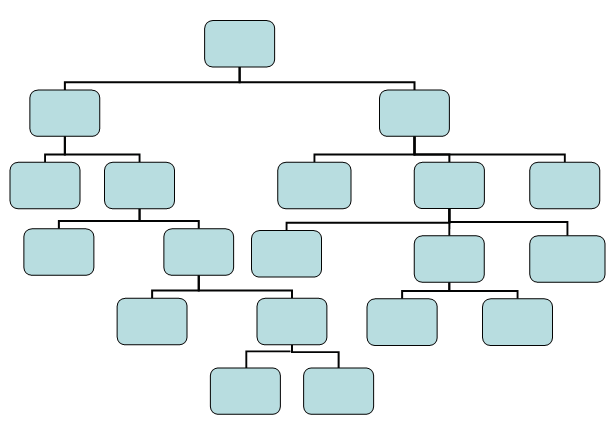
\includegraphics[width=0.85\linewidth]{img/fig9-4a-hierarchy.png}
        \par\vspace{4pt}{\small (a) Cấu trúc phân cấp mẫu}
    \end{minipage}\hfill
    \begin{minipage}{0.48\linewidth}
        \centering
        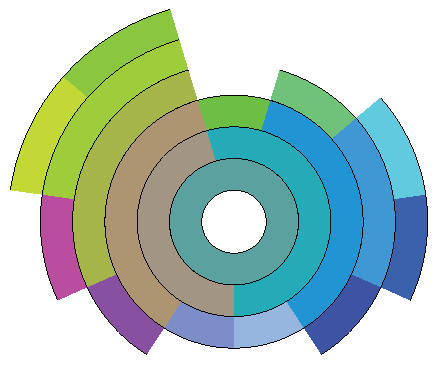
\includegraphics[width=0.85\linewidth]{img/fig9-4b-sunburst.png}
        \par\vspace{4pt}{\small (b) Biểu đồ sunburst tương ứng}
    \end{minipage}
    \caption{Một cấu trúc phân cấp mẫu và biểu đồ sunburst tương ứng.}
    \label{fig:sunburst}
\end{figure}

\FloatBarrier
\section*{9.1.2. Các phương pháp không lấp đầy không gian}
\addcontentsline{toc}{section}{Phần 9.1.2. Các phương pháp không lấp đầy không gian}

\subsubsection{Sơ đồ node-link cho cấu trúc cây}

Cách biểu diễn phổ biến nhất dùng để trực quan hóa quan hệ cây hay quan hệ phân cấp là sơ đồ node-link. Sơ đồ tổ chức, cây gia phả và bảng ghép cặp thi đấu chỉ là một vài trong số những ứng dụng thường gặp của loại sơ đồ này. Việc vẽ những cây như vậy chịu ảnh hưởng nhiều nhất bởi hai yếu tố: bậc phân nhánh \footnote{Số node anh em mà một node cha có thể có} và độ sâu \footnote{Node nằm xa node gốc nhất}. Những cây bị ràng buộc chặt ở một hoặc cả hai khía cạnh này (chẳng hạn cây nhị phân, hay cây chỉ có ba đến bốn tầng) thường dễ vẽ hơn nhiều so với những cây ít bị ràng buộc hơn.

Khi thiết kế thuật toán vẽ bất kỳ sơ đồ node-link nào (không riêng gì cây), ta phải cân nhắc ba nhóm nguyên tắc thường mâu thuẫn với nhau: quy ước vẽ, ràng buộc và tính thẩm mỹ. Các quy ước có thể bao gồm việc giới hạn cạnh chỉ được là một đoạn thẳng đơn, một chuỗi các đoạn thẳng vuông góc, các đường gấp khúc đa giác, hoặc các đường cong. Những quy ước khác có thể là đặt các node trên một lưới cố định, hoặc buộc mọi node anh em phải có cùng vị trí theo phương dọc. Các ràng buộc có thể bao gồm yêu cầu một node cụ thể phải nằm ở tâm màn hình, hoặc một nhóm node phải được đặt gần nhau, hoặc một số liên kết nhất định bắt buộc phải đi từ trên xuống dưới hoặc từ trái sang phải. Mỗi nguyên tắc nêu trên đều có thể được dùng để dẫn dắt việc thiết kế thuật toán.

Tuy nhiên, tính thẩm mỹ thường có tác động đáng kể đến khả năng diễn giải của một hình vẽ cây hay đồ thị, song lại thường dẫn đến những nguyên tắc xung đột nhau\footnote{Trong lĩnh vực vẽ đồ thị, việc tối ưu hóa đồng thời các tiêu chí thẩm mỹ (đặc biệt là cực tiểu hóa số giao cắt cạnh) trên đồ thị tổng quát là bài toán thuộc lớp NP-khó. Tuy nhiên, đối với cấu trúc cây phân cấp, các thuật toán kinh điển như Reingold--Tilford (1981) hay Walker (1990) có thể đạt được tính thẩm mỹ cao và đối xứng với độ phức tạp thời gian tuyến tính $O(|V|)$ và không có cạnh nào bị cắt nhau.}. Một số quy tắc thẩm mỹ điển hình bao gồm:

\begin{itemize}
    \item giảm thiểu số giao cắt đường,
    \item duy trì một tỉ lệ khung hình dễ nhìn,
    \item giảm thiểu tổng diện tích của hình vẽ,
    \item giảm thiểu tổng độ dài các cạnh,
    \item giảm thiểu số điểm gấp khúc trên các cạnh,
    \item giảm thiểu số lượng góc hoặc độ cong khác nhau được sử dụng,
    \item hướng tới một cấu trúc đối xứng.
\end{itemize}

Đối với cây, đặc biệt là cây cân bằng, việc thiết kế thuật toán tuân thủ nhiều (nếu không muốn nói là hầu hết) các nguyên tắc trên là tương đối dễ dàng. Chẳng hạn, một thủ tục vẽ cây đơn giản được trình bày dưới đây (kết quả mẫu được thể hiện ở Hình \ref{fig:nodelink}):

\begin{enumerate}
    \item Cắt vùng vẽ thành các dải có chiều cao bằng nhau, dựa trên độ sâu của cây.
    \item Với mỗi tầng của cây, xác định cần vẽ bao nhiêu node.
    \item Chia mỗi dải thành các hình chữ nhật có kích thước bằng nhau, dựa trên số node ở tầng đó.
    \item Vẽ mỗi node vào tâm hình chữ nhật tương ứng của nó.
    \item Vẽ một liên kết từ điểm giữa cạnh dưới của mỗi node đến điểm giữa cạnh trên của (các) node con của nó.
\end{enumerate}

\begin{figure}[htbp]
    \centering
    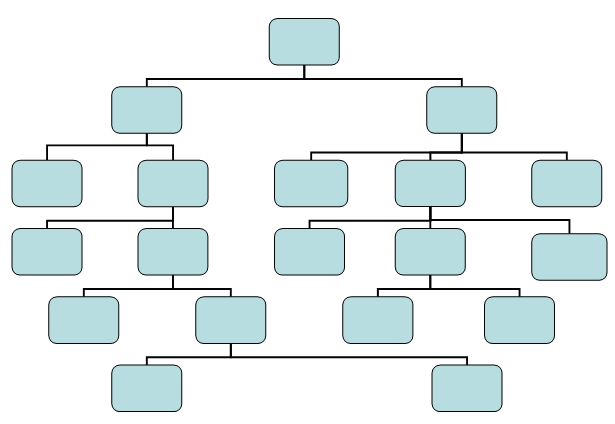
\includegraphics[width=0.65\linewidth]{img/fig9-5-node-link.png}
    \caption{Một ví dụ trực quan hóa cấu trúc phân cấp bằng sơ đồ node-link đơn giản, sử dụng khoảng cách đều nhau ở mỗi tầng.}
    \label{fig:nodelink}
\end{figure}

Có thể thực hiện nhiều cải tiến cho thuật toán khá cơ bản này nhằm nâng cao hiệu quả sử dụng không gian và đưa các node con lại gần node cha hơn. Một số cải tiến đó gồm:

\begin{itemize}
    \item Thay vì dùng khoảng cách đều và căn giữa, hãy chia mỗi tầng dựa trên số node lá thuộc về mỗi cây con.
    \item Trải đều các node lá trên toàn vùng vẽ và căn các node cha vào chính giữa, phía trên chúng.
    \item Thêm một khoảng đệm giữa các node liền kề không phải anh em để làm nổi bật quan hệ.
    \item Nếu có thể, sắp xếp lại thứ tự các cây con của một node để đạt được độ đối xứng và cân đối cao hơn.
    \item Đặt node gốc ở tâm màn hình và bố trí các node con theo hướng xuyên tâm, thay vì theo phương dọc.
\end{itemize}

\FloatBarrier
\subsubsection{Hiển thị trong không gian ba chiều}

Đối với những cây lớn, một hướng tiếp cận phổ biến là sử dụng chiều thứ ba, bổ sung thêm các công cụ xoay, tịnh tiến và thu phóng. Kỹ thuật nổi tiếng nhất trong số đó được gọi là cây hình nón [341]\footnote{Mặc dù là một bước đột phá trong trực quan hóa tương tác 3D lúc bấy giờ, trong thực tiễn người ta vẫn ưa chuộng các cấu trúc cây 2D hơn, bởi vì không gian 3D dễ gặp hiện tượng các nhánh phía trước che khuất các node quan trọng phía sau.}. Trong bố cục này, các node con của một node được sắp xếp theo hướng xuyên tâm tại những góc cách đều nhau, rồi được dịch chuyển theo phương vuông góc với mặt phẳng. Hai tham số then chốt của quá trình này là bán kính và khoảng dịch chuyển; thay đổi chúng sẽ ảnh hưởng đến mật độ của hình hiển thị và mức độ che khuất. Ở mức tối thiểu, chúng phải được đặt sao cho các nhánh riêng biệt của cây không rơi vào cùng một vùng của không gian ba chiều. Một cách để bảo đảm điều này là cho bán kính tỉ lệ nghịch với độ sâu của node trong cây. Theo cách đó, những node gần node gốc sẽ được tách xa nhau đáng kể, còn những node ở gần đáy cây thì nằm sát nhau hơn. Một ví dụ được thể hiện ở Hình \ref{fig:conetree}.

\begin{figure}[htbp]
    \centering
    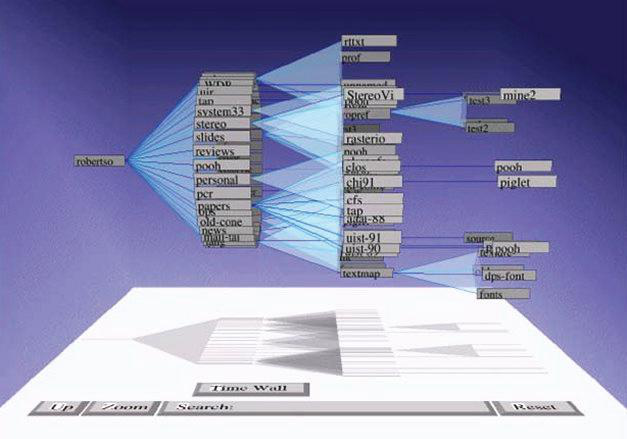
\includegraphics[width=0.75\linewidth]{img/fig9-6-cone-tree.png}
    \caption{Một ví dụ về cấu trúc phân cấp được hiển thị bằng cone tree [341]. (Hình ảnh \copyright~1991 Association of Computing Machinery. In lại với sự cho phép, do PARC, Inc. cung cấp.)}
    \label{fig:conetree}
\end{figure}

\chapter*{Phần 9.2. \newline Biểu diễn Đồ thị, Mạng tùy ý}
\addcontentsline{toc}{chapter}{Phần 9.2. Biểu diễn Đồ thị, Mạng tùy ý}
\markboth{Phần 9.2. Biểu diễn Đồ thị, Mạng tùy ý}{}

Cây chỉ là một dạng của một cách biểu diễn quan hệ tổng quát hơn, gọi là đồ thị. Nói một cách chính xác về mặt kỹ thuật, cây là một đồ thị liên thông, không trọng số và không có chu trình. Rõ ràng còn rất nhiều khả năng khác nữa, bao gồm đồ thị có cạnh mang trọng số, đồ thị vô hướng, đồ thị có chu trình, đồ thị không liên thông, v.v. Thay vì đưa ra thêm các thuật toán dành riêng cho từng lớp đồ thị khác nhau, cuốn sách mô tả một số hướng tiếp cận tổng quát để trực quan hóa những đồ thị mà ta không biết trước lớp hay cấu trúc của nó; ta gọi đó là đồ thị tùy ý. 

Trong phạm vi trình bày ở đây, ta giả định đồ thị là vô hướng, mặc dù một số kỹ thuật được nêu có thể mở rộng dễ dàng sang đồ thị có hướng. Ta sẽ xem xét hai hướng vẽ đồ thị tách biệt nhau: sơ đồ node-link (tiếp nối phần đã trình bày ở mục trước) và hiển thị dạng ma trận. Các tài liệu rộng và sâu hơn về vẽ đồ thị sẽ được giới thiệu ở cuối chương.

Một số đồ thị khá phức tạp [85, 239]. Chẳng hạn, các đồ thị trong thế giới thực hay còn được gọi phổ biến hơn là mạng, chúng có những đặc trưng ít khi tìm thấy ở các mạng đơn giản hay mạng ngẫu nhiên. Mạng thực tế có nhiều nhóm rời rạc, không liên thông với nhau, kích thước rất khác nhau; bậc của các node tuân theo luật lũy thừa \footnote{Tức sẽ chứa một lượng nhỏ các node có bậc cực lớn trong khi phần lớn các node có bậc tương đối nhỏ}; và đường kính \footnote{Đường kính của mạng là khoảng cách ngắn nhất dài nhất giữa hai node trong mạng. Để tính đường kính đồ thị, ta tìm đường đi ngắn nhất có thể giữa các cặp đỉnh trong đồ thị, thu được một tập hợp các đường đi, trong đó độ dài của đường dài nhất chính là độ lớn đường kính của đồ thị.} của mạng bị giới hạn nếu so với các đồ thị ngẫu nhiên tương đương có cùng số node và số cạnh [7, 311]. Tính chất trên là hệ quả của tính chất về bậc của các node, các điểm có bậc cực lớn đóng vai trò là đường đi trung gian tối ưu cho phần lớn các trường hợp, từ đó góp phần giảm đường kính đồ thị.

Strogatz [401] mô tả những cách khác nhau khiến một đồ thị bộc lộ tính phức tạp, bao gồm: phức tạp về cấu trúc (các cạnh rối vào nhau), sự tiến hóa của mạng (mạng biến đổi theo thời gian), sự đa dạng của kết nối (trọng số/hướng), phức tạp về động lực (trạng thái của node thay đổi theo thời gian), và sự đa dạng của node (có nhiều loại node khác nhau).

\section*{9.2.1. Đồ thị Node-Link}
\addcontentsline{toc}{section}{Phần 9.2.1. Đồ thị Node-Link}

\subsubsection{Phương pháp force-directed} 

Các phương pháp vẽ đồ thị force-directed (định hướng bằng lực) dùng phép so sánh với lò xo để biểu diễn các liên kết: vị trí của các node được tinh chỉnh lặp đi lặp lại cho đến khi tổng năng lượng (hay ứng suất) của hệ đạt cực tiểu. Với mỗi cặp node có liên kết, tồn tại hai lực: $f_{ij}$, lực gây ra bởi lò xo nối chúng, và $g_{ij}$, lực đẩy tĩnh điện có tác dụng giữ cho các node không tiến lại quá gần nhau. Một mô hình đơn giản là dùng định luật Hooke cho lực lò xo và định luật nghịch đảo bình phương cho lực đẩy. Hình \ref{fig:spring} minh họa hai lực này tác động lên hai node $i$ và $j$.

\begin{figure}[h]
    \centering
    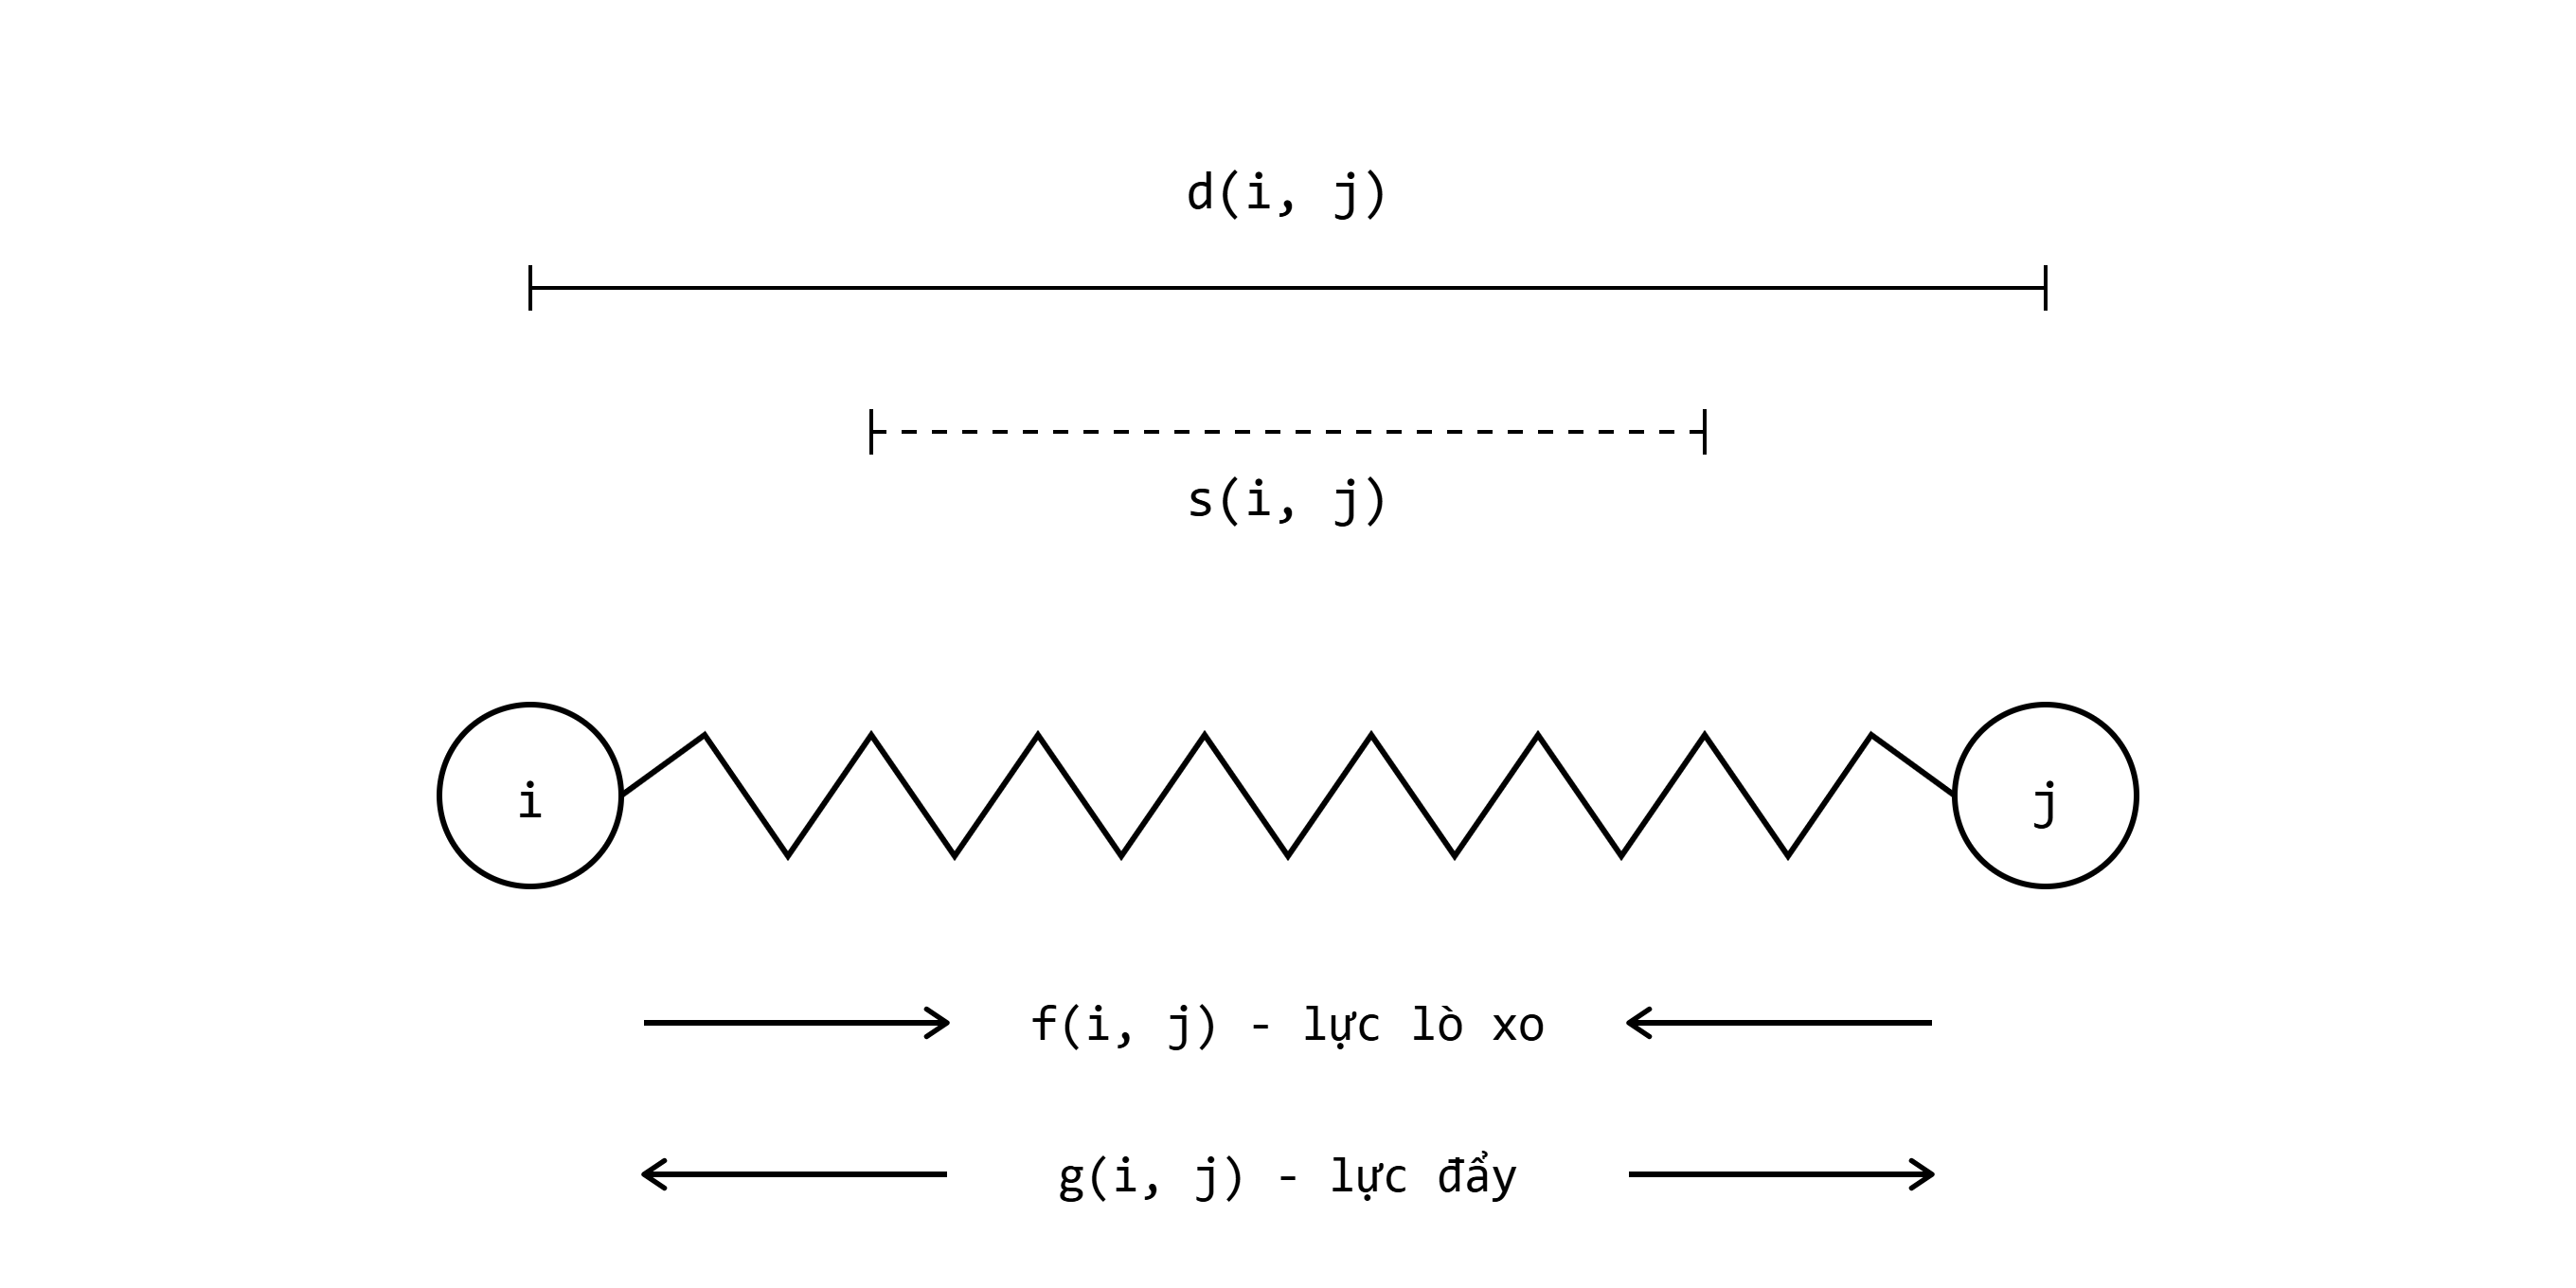
\includegraphics[width=\textwidth]{img/spring_force_diagram_white_bg_fixed.png}
    \caption{Lò xo đang bị kéo dãn ($d > s$) nên lực $f$ kéo hai node lại gần, trong khi lực đẩy $g$ tỉ lệ nghịch với $d_2$ thì luôn đẩy chúng ra xa. Vị trí cân bằng là nơi hai lực triệt tiêu nhau.}
    \label{fig:spring}
\end{figure}

Gọi $d(i, j)$ là khoảng cách Euclid giữa node $i$ và node $j$, $s_{i,j}$ là chiều dài tự nhiên của lò xo khi ở trạng thái nghỉ, và $k_{ij}$ là độ căng của lò xo, thì thành phần theo trục $x$ của lực lò xo giữa hai node được tính bằng:

\begin{equation}
f_{ij}(x) = k_{ij} \cdot \big(d(i,j) - s_{ij}\big) \cdot \frac{x_i - x_j}{d(i,j)} 
\label{equa:Hooke}
\end{equation}

Nếu $r_{ij}$ là cường độ của lực đẩy giữa node $i$ và node $j$, thành phần theo trục $x$ của lực đẩy được tính bằng:

\begin{equation}
g_{ij}(x) = \frac{r_{ij}}{d(i,j)^2} \cdot \frac{x_i - x_j}{d(i,j)}
\label{equa:tinhdien}
\end{equation}

Về bản chất, cả hai lực trên là các đại lượng vector hướng theo đường thẳng
nối hai node $i$ và $j$. Gọi
\[
  \vec{u}_{ij} = \frac{(x_i - x_j,\ y_i - y_j)}{d(i,j)}
\]
là vector đơn vị chỉ từ $j$ sang $i$, thì lực lò xo và lực đẩy có dạng
vector đầy đủ:
\[
  \vec{F}_{ij} = k_{ij} \cdot \big(d(i,j) - s_{ij}\big) \cdot \vec{u}_{ij},
  \qquad
  \vec{G}_{ij} = \frac{r_{ij}}{d(i,j)^2} \cdot \vec{u}_{ij}.
\]
Vì thuật toán bố trí đồ thị cập nhật tọa độ theo từng trục riêng biệt, ta
cần chiếu các vector lực này lên trục $x$, bằng cách nhân độ lớn của lực
với thành phần $x$ của $\vec{u}_{ij}$, chính là $\frac{x_i - x_j}{d(i,j)}$.
Đó là lý do công thức \ref{equa:Hooke} và \ref{equa:tinhdien} đều xuất hiện thừa số
$\frac{x_i - x_j}{d(i,j)}$ ở cuối; muốn có thành phần theo trục $y$ chỉ
cần thay $x_i - x_j$ bằng $y_i - y_j$.

Mỗi bước của quá trình tinh chỉnh vị trí sẽ tính tổng tất cả các lực tác dụng lên mỗi node (các thành phần theo $x$, $y$, và $z$ tùy trường hợp) rồi dịch chuyển vị trí của node đó một lượng tỉ lệ với lực tổng hợp ấy. Hiển nhiên là một khi các điểm đã di chuyển thì toàn bộ các lực phải được tính lại và lại thực hiện một lần dịch chuyển vị trí nữa. Để tránh hiện tượng dao động \footnote{Hiện tượng khi các node di chuyển qua lại một vị trí nhất định. Xảy ra khi bài toán tối ưu (ở đây là tối thiểu lực tác động lên hệ) rơi vào cực tiểu cục bộ. Hiện tượng này khá tương đồng với hiện tượng đảo chiều liên tục của gradient qua các bước cập nhật trong huấn luyện mô hình học máy.}, thông thường người ta bắt đầu bằng những bước dịch chuyển chiếm một tỉ lệ đáng kể so với lực, rồi giảm dần kích thước bước để hội tụ về điểm mà tại đó các lực đạt cực tiểu. Vị trí ban đầu có thể được gán ngẫu nhiên. Vì hoàn toàn có khả năng kết thúc ở một cực tiểu năng lượng cục bộ thay vì cực tiểu toàn cục, người ta thường chạy thuật toán bố trí nhiều lần với các cấu hình khởi tạo khác nhau để chọn ra cấu hình tốt nhất trong số các cấu hình đã tính được. Độ tốt của một cách bố trí có thể được tính dựa trên tổng độ lớn của các lực trên cấu hình đó.

\subsubsection{Vẽ đồ thị phẳng}

Các kỹ thuật vẽ đồ thị phẳng xuất phát từ giả định rằng đồ thị nền là phẳng, tức là nó không có cạnh nào cắt nhau. Những thuật toán này nhận được rất nhiều sự chú ý vì vài lý do. Thứ nhất, do lý thuyết về đồ thị phẳng đã có bề dày lịch sử lâu đời, có rất nhiều khái niệm có thể khai thác được từ kho tài liệu sẵn có. Thứ hai, vì các cạnh cắt nhau thường làm đồ thị trở nên khó đọc, việc giảm thiểu hoặc loại bỏ hoàn toàn những chỗ cắt nhau đó là một chiến lược tốt. Cuối cùng, đồ thị phẳng thường thưa: công thức Euler chỉ ra rằng một đồ thị phẳng có $n$ đỉnh thì có nhiều nhất $3n − 6$ cạnh. Việc tập trung vào đồ thị phẳng cũng không quá hạn chế, bởi ta có thể loại bỏ các điểm cắt bằng cách chèn node giả vào ngay tại các điểm cắt đó, thực hiện bố trí bằng thuật toán dành cho đồ thị phẳng, rồi sau đó gỡ bỏ các node giả đi.

Ngoài ra, ta còn giả định rằng đồ thị là liên thông, tức là tồn tại một đường đi từ mọi node đến mọi node khác. Những đồ thị không liên thông có thể được tách thành các đồ thị con và vẽ riêng rẽ. Một đồ thị con liên thông cực đại (tất cả các node đều nối được với nhau) chính là một thành phần liên thông của đồ thị. Một số định nghĩa hữu ích khác gồm:

\begin{itemize}
    \item Một mặt (face) là một phần của mặt phẳng được cô lập bởi một tập các đỉnh liên thông với nhau.
    \item Một tập lân cận là danh sách các đỉnh kề với một đỉnh cụ thể, liệt kê theo chiều ngược chiều kim đồng hồ.
    \item Một phép nhúng phẳng là một lớp các cách vẽ đồ thị phẳng có cùng tập lân cận cho mỗi đỉnh. Một đồ thị phẳng có thể có số phép nhúng như vậy lớn tới cấp hàm mũ.
    \item Một đỉnh khớp là node bất kỳ mà khi bị loại bỏ sẽ làm đồ thị mất liên thông.
    \item Một đồ thị song liên thông (biconnected graph) là đồ thị không có đỉnh khớp nào.
    \item Một khối là một đồ thị con song liên thông cực đại của một đồ thị.
    \item Một cặp phân tách là hai đỉnh mà khi bị loại bỏ sẽ làm một đồ thị song liên thông trở nên mất liên thông.
    \item Một đồ thị tam liên thông (triconnected graph) là đồ thị không có cặp phân tách nào. Một đồ thị phẳng tam liên thông có phép nhúng duy nhất.
\end{itemize}

Trước hết ta cần một chiến lược để xác định xem một đồ thị có phẳng hay không. Đã có vài thuật toán như vậy, tuy nhiên những thuật toán hiệu quả thì lại có độ phức tạp rất cao, còn những thuật toán đơn giản thì thường tốn kém về mặt tính toán. Ta có thể bắt đầu bằng cách đơn giản hóa bài toán đi một chút. Ta làm điều đó bằng nhận xét rằng một đồ thị là phẳng chỉ khi tất cả các thành phần liên thông của nó cũng phẳng. Tương tự, ta có thể phát biểu rằng một đồ thị liên thông là phẳng chỉ khi mọi thành phần song liên thông của nó đều phẳng. Như vậy, ta chỉ cần một thuật toán xác định xem một đồ thị song liên thông có phẳng hay không.

Lập luận tổng quát của thuật toán như sau. Ta sẽ áp dụng cách tiếp cận chia để trị, dựa trên nhận xét: nếu đồ thị của ta chứa một chu trình sao cho không tồn tại chu trình nào khác mà không chứa ít nhất một cạnh của chu trình ban đầu (tức là khi gỡ bỏ các cạnh thuộc chu trình ban đầu thì không còn chu trình nào sót lại), thì phần còn lại chỉ là những đường đi bắt đầu và kết thúc tại các đỉnh của chu trình (các đỉnh này được gọi là điểm gắn). Những mảnh này của đồ thị có thể được vẽ hoặc ở bên trong chu trình, hoặc ở bên ngoài chu trình. Hai mảnh được gọi là đan chéo nhau nếu cả hai đều bắt đầu và kết thúc trên các node của chu trình, và hai đầu mút của mảnh này bị ngăn cách bởi một đầu mút của mảnh kia. Để vẽ được theo cách phẳng, một trong hai mảnh đan chéo đó phải được vẽ bên trong chu trình, còn mảnh kia phải vẽ bên ngoài. Bây giờ, nếu ta dựng một đồ thị gồm tất cả các mảnh, trong đó có một cạnh nối hai mảnh nếu chúng đan chéo nhau, thì chừng nào đồ thị này còn là đồ thị hai phía, tức là tách được thành hai tập đỉnh sao cho không tồn tại cạnh nào nối hai phần tử thuộc cùng một tập thì đồ thị ban đầu là phẳng. Hình \ref{fig:planar} là một cách vẽ phẳng của đồ thị trong ví dụ ở Hình \ref{fig:biconnected}.

\begin{figure}
    \centering
    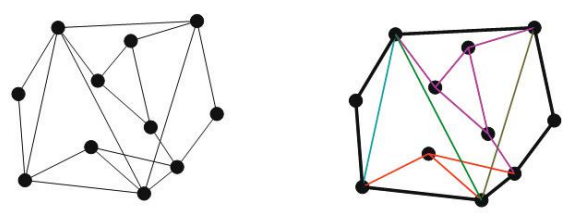
\includegraphics[width=1\linewidth]{img/sample_graph.png}
    \caption{Một ví dụ về đồ thị song liên thông, chu trình được minh họa bằng màu đen đậm và năm mảnh với các màu khác nhau.}
    \label{fig:biconnected}
\end{figure}

\begin{figure}
    \centering
    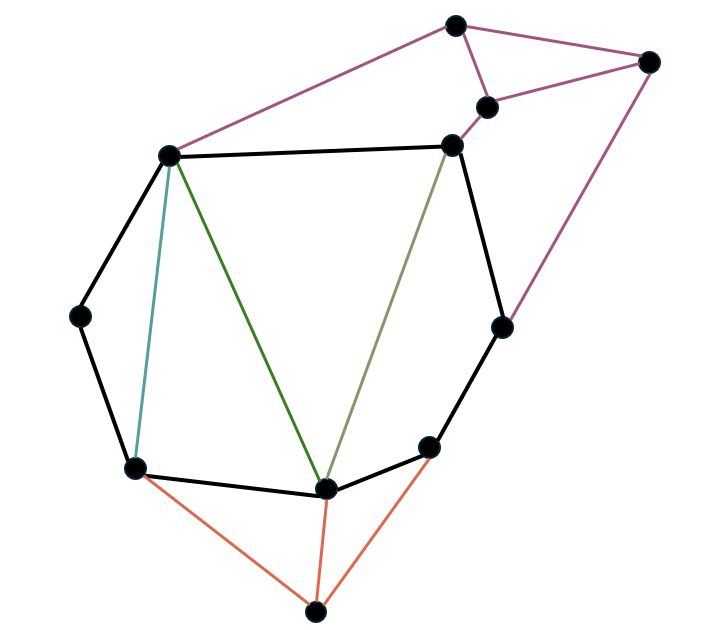
\includegraphics[width=0.5\linewidth]{img/planar.png}
    \caption{Một cách phẳng hóa của đồ thị trong ví dụ ở Hình \ref{fig:biconnected}.}
    \label{fig:planar}
\end{figure}

Nếu sau khi gỡ bỏ các cạnh của chu trình ban đầu mà đồ thị vẫn còn chứa chu trình, điều đó có nghĩa là một hoặc nhiều mảnh trong số đó bản thân chúng có chứa chu trình (xem mảnh màu tím trong Hình \ref{fig:biconnected} và Hình \ref{fig:planar}). Trong trường hợp này, ta tạo một đồ thị con gồm mảnh đó cộng với một đoạn của chu trình ban đầu nối hai đầu mút của mảnh, rồi gọi đệ quy thuật toán kiểm tra tính phẳng. Mã giả của thuật toán như sau [27]. Lưu ý rằng chu trình phân tách là chu trình sinh ra ít nhất hai mảnh.

Cho một đồ thị song liên thông G và một chu trình phân tách C:

\begin{enumerate}
    \item Tính tất cả các mảnh của $G$ ứng với $C$.

    \item Với mỗi mảnh $P$ không phải là một đường đi đơn:
    \begin{enumerate}
        \item Tạo đồ thị $G'$ gồm $P$ cộng với $C$.

        \item Tạo chu trình $C'$ gồm một đường đi xuyên qua $P$
        cộng với đoạn của $C$ nối hai đầu mút đó.

        \item Áp dụng thuật toán cho $(G', C')$.
        Nếu kết quả là không phẳng thì $G$ không phẳng.
    \end{enumerate}

    \item Tính đồ thị đan chéo $I$ của các mảnh của $G$.

    \item Nếu $I$ không phải là đồ thị hai phía thì $G$ không phẳng;
    ngược lại $G$ là phẳng.
\end{enumerate}

Nếu một đồ thị không phẳng, ta có thể làm cho nó trở nên phẳng bằng chiến lược sau:

\begin{enumerate}
    \item Xác định đồ thị con phẳng lớn nhất của đồ thị.
    \item Với các đỉnh còn lại, đặt mỗi đỉnh vào một mặt sao cho số cạnh cắt nhau là nhỏ nhất.
    \item Với mỗi chỗ cạnh cắt nhau, tách mỗi cạnh thành hai phần và nối các đầu vừa bị tách vào một đỉnh giả mới.
\end{enumerate}

\subsubsection{Phương pháp visibility}

Một khi đồ thị đã được xác định là phẳng, hoặc đã được bổ sung để đạt được tính phẳng, có rất nhiều chiến lược khả dĩ để sinh ra một bản vẽ. Một kỹ thuật như vậy, gọi là phương pháp visibility [27], gồm một quy trình hai bước.

Ở bước thứ nhất, gọi là bước visibility, ta dựng nên một biểu diễn visibility của đồ thị. Trong cách biểu diễn này, mỗi đỉnh được vẽ thành một đoạn thẳng nằm ngang, còn mỗi cạnh được vẽ thành một đường thẳng đứng nối các đoạn thẳng đỉnh tương ứng. Có thể thấy rõ rằng với một đồ thị phẳng, ta luôn luôn vẽ được một biểu diễn như vậy mà các cạnh không cắt nhau ở đâu ngoài chính những chỗ chúng gặp các đoạn thẳng đỉnh. Hiển nhiên là có rất nhiều thứ tự sắp xếp khả dĩ cho các đoạn thẳng đỉnh; một chiến lược có thể dùng là sắp xếp chúng sao cho tổng chiều dài của các đường nối thẳng đứng là nhỏ nhất.

Ở bước thứ hai, gọi là bước thay thế, mỗi đoạn thẳng đỉnh được co lại thành một điểm duy nhất, và mỗi đường nối thẳng đứng được thay bằng một đường gấp khúc bám theo cạnh gốc nhiều nhất có thể, với một đoạn ở mỗi đầu để nối cạnh đó với đỉnh tương ứng của nó. Có nhiều lựa chọn cho bước thay thế, bao gồm vị trí đặt các node và chiến lược tạo các đường nối (ví dụ: đường thẳng hay đường cong, một đoạn duy nhất hay nhiều đoạn).

\begin{figure}
    \centering
    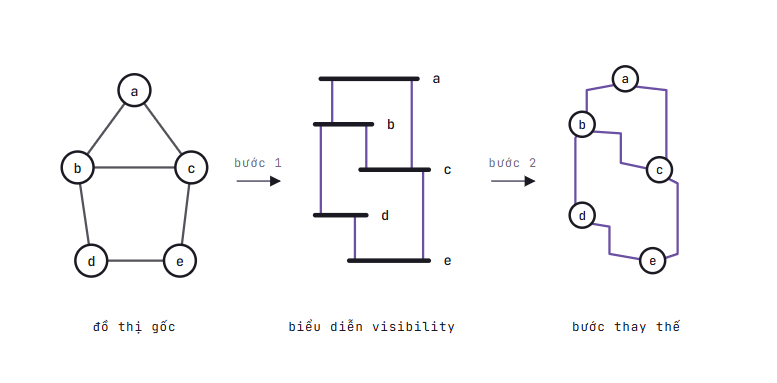
\includegraphics[width=1\linewidth]{img/visibility.png}
    \caption{Cùng một đồ thị năm đỉnh qua ba giai đoạn. Ở giữa, mỗi đỉnh thành một đoạn nằm ngang và mỗi cạnh thành một đường thẳng đứng: cạnh $a–c$ đi lọt qua mức của $b$ đúng vì đoạn của $b$ không vươn tới cột đó, thể hiện tính "nhìn thấy nhau" của biểu diễn này. Bên phải, mỗi đoạn co về một điểm và mỗi đường nối thành một đường gấp khúc ba đoạn.}
    \label{fig:visibility}
\end{figure}

\subsubsection{Mạng phức tạp}

Renoust [332] mô tả một cách phân tích mạng đa lớp. Ông định nghĩa một độ đo về mức độ quấn bện vào nhau của các cạnh (chỉ số đan bện), từ đó dẫn tới các độ đo khác (ví dụ: cường độ, và tính đồng nhất) và cuối cùng dẫn tới việc hiểu được mạng tương tác chất xúc tác.

Mạng thì rất đa dạng. Mạng phức tạp đã được nghiên cứu từ lâu, và việc mô tả đặc trưng cũng như định nghĩa chúng đến nay vẫn còn là chủ đề của nhiều công bố [85, 239]. Tuy vậy, ta có thể thừa nhận rằng mạng phức tạp là mạng thể hiện những đặc trưng mà ta không tìm thấy ở mạng đơn giản cũng như ở mạng ngẫu nhiên, nhưng lại rất thường gặp ở các mạng trong thế giới thực [452]. Cụ thể hơn về mặt thực nghiệm, các tài liệu đã phát hiện [7] và vẫn đang tiếp tục phát hiện [311] những đặc trưng của mạng phức tạp trong hầu hết các mạng thực tế. Trong số các đặc trưng đó, nổi tiếng nhất là [7]:

\begin{itemize}
    \item Dáng vẻ thế giới nhỏ: đường kính của mạng khá hạn chế nếu so với đường kính của một đồ thị ngẫu nhiên có cùng số node và số cạnh;
    \item Phân bố bậc không phụ thuộc thang đo: người ta quan sát thấy một cái đuôi dài trong phân bố bậc của các node, thường được nhắc đến với tên gọi luật lũy thừa;
    \item Hệ số phân cụm cao: hệ số phân cụm ở mạng thực tế cao hơn nhiều so với ở mạng ngẫu nhiên.
\end{itemize}

Một mạng phức tạp thể hiện ít nhất một vài trong số các đặc trưng trên và các đặc trưng ấy không chỉ giới hạn ở những gì vừa nêu [78]. Trong một đồ thị thực tế, ta cũng có thể quan sát thấy nhiều thành phần không liên thông với kích thước biến thiên rất mạnh (nhiều khả năng là do một đặc tính scale-free bên trong như mô tả ở trên gây ra). Một hoặc vài thành phần lớn nhất có thể thể hiện phần lớn các đặc trưng của mạng phức tạp.

Strogatz, trong công trình của mình [401], định nghĩa sáu cách khác nhau để một mạng bộc lộ tính phức tạp:

\begin{itemize}
    \item phức tạp về cấu trúc (các cạnh rối vào nhau),
    \item sự tiến hóa của mạng (mạng biến đổi theo thời gian),
    \item sự đa dạng của kết nối (trọng số/hướng/dấu của các cạnh),
    \item phức tạp về động lực (trạng thái node có thể thay đổi theo thời gian),
    \item sự đa dạng của node (có nhiều loại node khác nhau),
    \item siêu phức tạp (meta-complication).
\end{itemize}

\section*{9.2.2. Biểu diễn ma trận cho đồ thị}
\addcontentsline{toc}{section}{Phần 9.2.2. Biểu diễn ma trận cho đồ thị}

Một cách biểu diễn trực quan thay thế cho đồ thị là dùng ma trận kề, là một lưới $N × N$ (với $N$ là số node), trong đó vị trí ($i$, $j$) biểu thị sự tồn tại (hay không tồn tại) của một liên kết giữa node $i$ và node $j$. Đây có thể là một ma trận nhị phân, hoặc giá trị trong ô có thể biểu thị cường độ hay trọng số của liên kết giữa hai node. Phương pháp này khắc phục được một trong những vấn đề lớn nhất của sơ đồ node-link, đó là hiện tượng các cạnh cắt nhau mặc dù nó lại không mở rộng tốt cho các đồ thị có số node lớn (hàng nghìn). Bertin [34] là một trong những nhà nghiên cứu đầu tiên khảo sát sức mạnh của cách biểu diễn này, sử dụng các chiến lược sắp xếp lại thứ tự khác nhau để tổ chức các hàng và các cột nhằm làm lộ ra cấu trúc bên trong đồ thị. Tầm quan trọng của việc sắp xếp lại thứ tự thể hiện rõ trong Hình \ref{fig:origin_matrix}, trong đó mỗi ma trận đều biểu diễn cùng một đồ thị tám node. Hai clique bốn node hiện ra rất rõ ràng ở hiển thị thứ hai.

% \begin{figure}
%     \centering
%     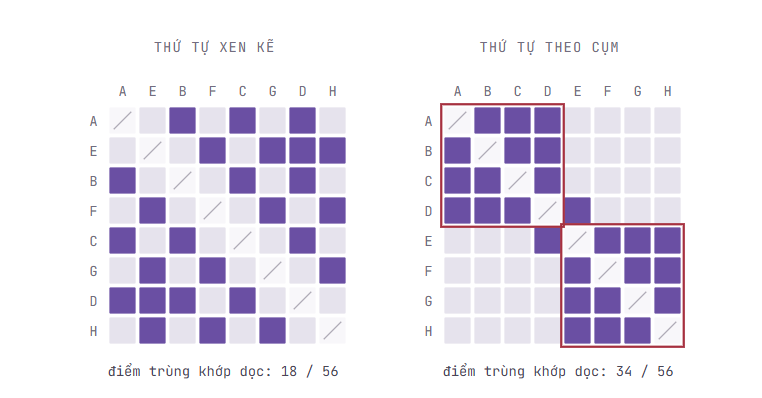
\includegraphics[width=1\linewidth]{img/matrix.png}
%     \caption{Đồ thị gồm hai clique bốn node \{A,B,C,D\} và \{E,F,G,H\} cùng một cạnh cầu D–E. Bên trái, hai clique được xếp xen kẽ nhau và cấu trúc biến mất; bên phải, chỉ đổi thứ tự chứ không đổi đồ thị, hai khối 4 × 4 hiện ra ngay. Chấm điểm bằng cách đếm số ô trùng khớp giữa các hàng kề nhau theo chiều dọc (tối đa 56): ma trận trái được 18, ma trận phải được 34. Sách dùng một đồ thị tám node khác và cho hai điểm số 9 và 20.}
%     \label{fig:matrix}
% \end{figure}

\begin{figure}
    \centering
    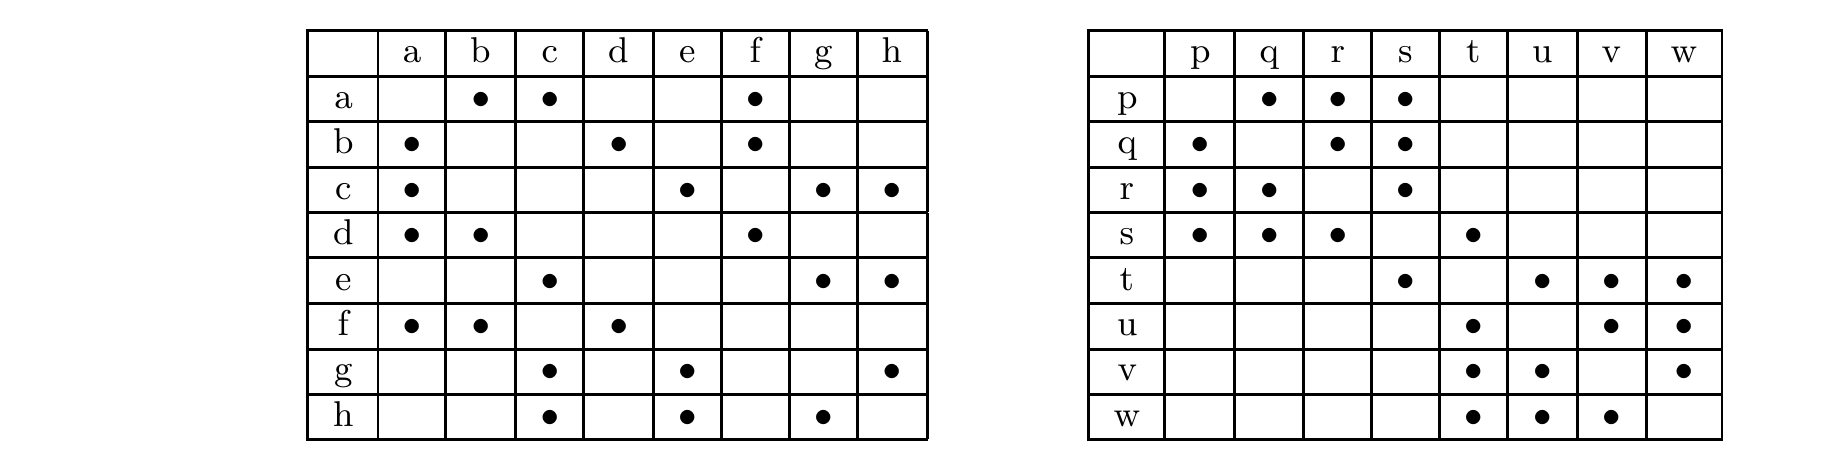
\includegraphics[width=1\linewidth]{img/origin_matrix.png}
    \caption{Hai cách hiển thị ma trận của cùng một đồ thị theo 2 thứ tự nodes khác nhau, cho thấy cấu trúc đồ thị hiểu thị rõ ràng hơn ở bên phải.}
    \label{fig:origin_matrix}
\end{figure}

Lấy ví dụ, ta có thể dùng một chiến lược đánh giá thứ tự hết sức đơn giản, đó là đếm số lần xuất hiện của các phần tử trùng khớp nhau ở những hàng hoặc cột kề nhau. Cách này có xu hướng gom lại với nhau những node cùng nối hoặc cùng không nối tới một node chung. Trong Hình \ref{fig:origin_matrix}, ma trận bên trái đạt điểm 9 khi chỉ đếm các cặp lân cận theo chiều dọc, trong khi ma trận bên phải đạt điểm 20. Bằng cách liệt kê tất cả các thứ tự khả dĩ, ta có thể tìm ra những thứ tự cho điểm trùng khớp cao nhất. Với số node vừa phải thì đây là một chiến lược chấp nhận được, nhưng vì số thứ tự khả dĩ là cỡ $N!$, cách tiếp cận này không mở rộng tốt. Việc sắp thứ tự các node tương tự như bài toán người du lịch (traveling salesman problem - TSP), trong đó ta cố tìm một hành trình đi qua một tập các thành phố mà không ghé thành phố nào quá một lần, đồng thời làm nhỏ nhất tổng quãng đường phải đi. Vì về cơ bản đây cũng chính là bài toán tìm thứ tự các hàng hoặc các cột của ma trận sao cho cực tiểu hóa một độ đo nào đó, nên các lời giải heuristic đã được dùng cho TSP cũng có thể áp dụng được ở đây.


\chapter*{Phần 9.3. \newline Các vấn đề khác}
\addcontentsline{toc}{chapter}{Phần 9.3. Các vấn đề khác}
\markboth{Phần 9.3. Các vấn đề khác}{}

Sau khi xây dựng được một hình thức trực quan hóa cơ bản cho một cây hoặc đồ thị, vẫn còn một số vấn đề bổ sung cần được xem xét, chủ yếu liên quan đến vấn đề khả năng diễn giải. Hai vấn đề quan trọng sẽ được trình bày chi tiết trong phần này là gắn nhãn và tương tác.

\subsection*{9.3.1 Gắn nhãn}
\addcontentsline{toc}{section}{9.3.1 Gắn nhãn}

Việc gắn nhãn phù hợp cho một hình thức trực quan hóa là rất quan trọng, giúp người xem hiểu được những gì đang được thể hiện. Một bản đồ sẽ có rất ít giá trị nếu không có một hình thức gắn nhãn nào đó; tương tự, một biểu đồ sử dụng mã hóa màu sẽ rất khó hiểu nếu không có chỉ dẫn về ý nghĩa tương ứng với các màu sắc. Trong trực quan hóa cây và đồ thị, vấn đề gắn nhãn trở nên phức tạp hơn, không chỉ vì có thể có rất nhiều nút, mà còn vì các nhãn có thể cần được đặt cho cả các liên kết giữa các nút.

Nếu chỉ có một số lượng nhỏ các nhãn phân biệt, chẳng hạn như khi biểu diễn loại liên kết hoặc một lớp được gán cho một nút, tốt nhất nên sử dụng các nhãn phi văn bản, chẳng hạn như màu sắc, kích thước hoặc hình dạng của nút; hoặc màu sắc, độ dày hay kiểu đường của liên kết. Cách này không đòi hỏi nhiều không gian trên màn hình và thông thường có thể được diễn giải một cách rõ ràng, ngay cả khi xuất hiện một mức độ giao cắt đường và che khuất nút vừa phải. Tuy nhiên, nếu số lượng nhãn phân biệt vượt quá năm hoặc sáu, khả năng xảy ra việc diễn giải sai có thể tăng lên đáng kể. Khi đó, cần có một chú giải để giải thích cách ánh xạ giữa các thuộc tính đồ họa và ý nghĩa của chúng.

Đối với các đồ thị nhỏ, một chiến lược phổ biến để gắn nhãn cho nút là đặt nhãn bên trong nút, sử dụng các nút có dạng hình chữ nhật hoặc hình bầu dục để có đủ không gian chứa văn bản. Để tránh làm sai lệch cảm nhận về các nút, kích thước của nút nên được quyết định dựa trên độ dài của nhãn dài nhất. Trong những trường hợp nhãn có thể rất dài, một lựa chọn là sử dụng các dạng viết tắt hoặc các nhãn số, kết hợp với một chú giải để diễn giải. Người xem cuối cùng sẽ ghi nhớ được mối tương ứng giữa các nhãn rút gọn và ý nghĩa thực tế của chúng. Một chiến lược tương tự cũng có thể được sử dụng để gắn nhãn cho cạnh, bằng cách đặt nhãn gần trung tâm của cạnh. Đối với các cạnh chủ yếu theo phương thẳng đứng, nhãn nên được đặt ở bên trái hoặc bên phải của cạnh; trong khi đối với các cạnh chủ yếu theo phương ngang, nhãn nên được đặt ở phía trên hoặc phía dưới. Việc sử dụng một chiến lược nhất quán sẽ làm giảm khả năng người xem vô tình gán một nhãn cho sai cạnh.

Ở một thái cực khác, nếu có một số lượng lớn các nhãn phân biệt cần được hiển thị, hoặc bản thân các nhãn khá dài, có thể dễ dàng nhận thấy rằng việc hiển thị đồng thời tất cả các nhãn sẽ không hiệu quả. Một số chiến lược đã được phát triển để giải quyết vấn đề này. Một giải pháp phổ biến là chỉ hiển thị các nhãn trong một vùng nhỏ của đồ thị, chẳng hạn như trong một bán kính nhất định xung quanh vị trí của con trỏ. Nếu mật độ hiển thị quá cao, có thể cần phải làm biến dạng hình thức trực quan hóa (xem tiểu mục tiếp theo) để cung cấp thêm không gian màn hình cho phần đồ thị đó. Một giải pháp thay thế cho việc làm biến dạng, đôi khi có hiệu quả, là xoay đồ thị để giảm sự chồng lấn giữa các nhãn (xem Hình \ref{fig:9.11}). Một giải pháp thú vị khác được đề xuất trong [48] là chỉ hiển thị một tập con ngẫu nhiên của các nhãn trong một khoảng thời gian ngắn, sau đó chuyển sang hiển thị các nhãn thuộc một tập con khác. Ý tưởng đằng sau cách tiếp cận này là trí nhớ ngắn hạn của người xem sẽ cho phép họ ghi nhớ được số lượng nhãn lớn hơn so với khi tất cả các nhãn được hiển thị tĩnh cùng một lúc, đặc biệt khi trí nhớ này được củng cố bằng cách làm mới thông tin một cách thường xuyên.

\begin{figure}[htbp]
    \centering
    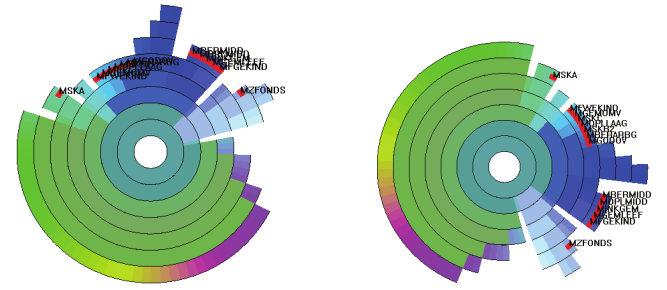
\includegraphics[width=0.85\textwidth]{img/k1.png}
    \caption{Cải thiện khả năng đọc của các nhãn bằng cách xoay đồ thị.}
    \label{fig:9.11}
\end{figure}

\subsection*{9.3.2 Tương tác}
\addcontentsline{toc}{section}{9.3.2 Tương tác}

Mặc dù Chương 11 và Chương 12 của tài liệu này dành riêng cho các kỹ thuật tương tác trong môi trường trực quan hóa, vẫn có một số kỹ thuật tương tác đặc biệt phù hợp với trực quan hóa cây và đồ thị, và sẽ được trình bày trong chương này. Một số loại tương tác, chẳng hạn như di chuyển khung nhìn và thu phóng, là những thao tác phổ biến đối với hầu hết các loại hình trực quan hóa, do đó ở đây chúng chỉ được đề cập ngắn gọn để đảm bảo tính đầy đủ. Những kỹ thuật khác, chẳng hạn như focus+context, mặc dù có thể áp dụng cho nhiều dạng trực quan hóa, nhưng chủ yếu được phát triển trong lĩnh vực trực quan hóa cây và đồ thị, vì vậy sẽ được mô tả chi tiết hơn trong phần này.

\subsubsection*{Tương tác với camera ảo}

Các thao tác như di chuyển khung nhìn, thu phóng và xoay có thể được xem như những thay đổi đơn giản đối với camera ảo được sử dụng để quan sát hoặc ghi lại một phần của cảnh. Những thao tác này cho phép người xem từng bước xây dựng một mô hình nhận thức về các đối tượng trong cảnh và mối quan hệ giữa chúng. Các thao tác thuộc loại này thường được điều khiển thủ công. Tuy nhiên, cũng có thể sử dụng các kỹ thuật tự động, chẳng hạn như di chuyển xuyên qua cảnh dựa trên dữ liệu và tự động xoay các đối tượng 3D, để tạo ra và trình bày các góc nhìn một cách tự động.

\subsubsection*{Tương tác với các phần tử của đồ thị}

Hầu hết các tương tác thuộc loại này đều bắt đầu bằng một thao tác lựa chọn, trong đó một hoặc nhiều thành phần của đồ thị được cô lập để thực hiện một hành động nào đó, chẳng hạn như làm nổi bật, xóa, che khuất, di chuyển hoặc xem thông tin chi tiết. Ví dụ, để giảm sự rối mắt trong một đồ thị, người dùng có thể chọn một số nút và kéo chúng đến một khu vực ít bị chiếm dụng hơn trên màn hình, đồng thời vẫn duy trì các liên kết của chúng. Tương tự, người dùng có thể chọn và di chuyển hoặc thay đổi hình dạng của một liên kết để loại bỏ một điểm giao cắt hoặc cải thiện tính thẩm mỹ của đồ thị. Việc lựa chọn có thể bao gồm một đối tượng đơn lẻ, tất cả các đối tượng nằm trong một vùng hoặc trong một khoảng cách được xác định trước, hoặc một tập hợp các đối tượng thỏa mãn một tập các ràng buộc do người dùng chỉ định (ví dụ: tất cả các nút được kết nối trực tiếp với một nút cho trước). Một trong những vấn đề lớn nhất khi lựa chọn các phần tử trong đồ thị xuất hiện tại những vùng có mật độ cao của bản vẽ, nơi các phần tử nằm quá gần nhau khiến việc lựa chọn một cách rõ ràng và không gây nhầm lẫn trở nên khó khăn hoặc thậm chí không thể thực hiện được. Điều này cho thấy sự cần thiết của các loại tương tác khác, chẳng hạn như thu phóng hoặc các kỹ thuật biến dạng được mô tả ở các phần sau.

\subsubsection*{Tương tác với cấu trúc đồ thị}

Có hai nhóm tương tác hướng trực tiếp đến cấu trúc của đồ thị. Nhóm thứ nhất dẫn đến những thay đổi đối với chính cấu trúc đó. Ví dụ, việc sắp xếp lại các nhánh của một cây có thể làm bộc lộ những mối quan hệ mà cách sắp xếp ban đầu chưa thể hiện rõ. Việc vẽ lại một đồ thị với các trọng số khác nhau cho các ràng buộc có thể tạo ra những đồ thị giúp thực hiện một số nhiệm vụ nhất định dễ dàng hơn. Việc sắp xếp lại các cột hoặc hàng trong một hình thức trực quan hóa ma trận có thể làm xuất hiện những đặc trưng hoặc mối quan hệ mới trong dữ liệu. Các kỹ thuật thuộc nhóm này thường phụ thuộc rất cụ thể vào loại đồ thị đang được hiển thị.

Nhóm tương tác thứ hai liên quan đến cấu trúc đồ thị bao gồm các kỹ thuật được gọi là focus+context, trong đó một tập con được lựa chọn của cấu trúc (focus) được trình bày với mức độ chi tiết cao, trong khi phần còn lại của cấu trúc được hiển thị ở mức độ chi tiết thấp hơn nhằm giúp người xem duy trì được bối cảnh tổng thể (context). Các kỹ thuật này có mối liên hệ với thao tác di chuyển khung nhìn và thu phóng, nhưng có ưu điểm là không làm mất đi bối cảnh của toàn bộ cấu trúc. Phổ biến nhất trong số các kỹ thuật biến dạng này là nhiều biến thể của thấu kính mắt cá, trong đó các phần của hình thức trực quan hóa nằm trong vùng tập trung được phóng đại bằng cách sử dụng phép co giãn phi tuyến, trong khi các phần nằm ngoài vùng tập trung được thu nhỏ một cách tương ứng để vẫn duy trì sự hiện diện của chúng trên màn hình. Sự biến dạng này có thể được thực hiện trong không gian màn hình, tức là dựa trên các điểm ảnh, hoặc trong không gian cấu trúc, tức là dựa trên các thành phần của đồ thị. Trường hợp thứ hai thú vị hơn trong trực quan hóa đồ thị. Chẳng hạn, chúng ta có thể phóng đại một nhánh của cây đồng thời thu nhỏ các nhánh khác, hoặc phóng đại tất cả các liên kết nằm trong phạm vi ba kết nối tính từ một nút cụ thể để quan sát vùng lân cận của nút đó một cách chi tiết hơn. Một ví dụ về biến dạng trong không gian cấu trúc được minh họa trong Hình \ref{fig:9.12}, trong đó cây con màu xanh của Hình \ref{fig:9.11} được phóng đại theo góc nhằm tạo điều kiện thuận lợi hơn cho việc khám phá và lựa chọn tương tác.

\begin{figure}[htbp]
    \centering
    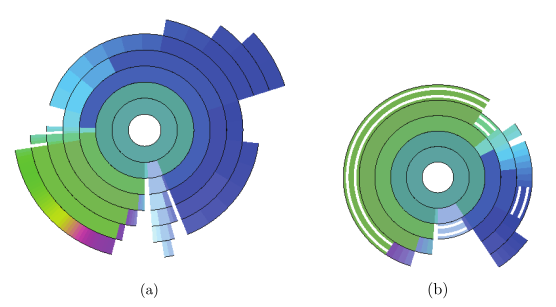
\includegraphics[width=0.85\textwidth]{img/k2.png}
    \caption{Một số thao tác tương tác trên các hình thức trực quan hóa sunburst: 
    (a) cây con màu xanh đã được mở rộng, trong khi phần còn lại của cây được thu gọn; 
    (b) một số cây con đã được thực hiện thao tác roll-up để đơn giản hóa hình thức hiển thị. 
    (Hình ảnh từ [481], \copyright~2003 Palgrave Macmillan.)}
    \label{fig:9.12}
\end{figure}

Một kỹ thuật có thể được xem là liên quan đến cả hai nhóm tương tác trên là ẩn hoặc loại bỏ có chọn lọc các phần của đồ thị. Ví dụ, sau khi một nhánh của cây đã được nghiên cứu một cách kỹ lưỡng, người dùng có thể muốn loại bỏ nhánh đó khỏi màn hình hiển thị để tạo thêm không gian cho những vùng chưa được khám phá. Theo một nghĩa nào đó, thao tác này có thể được xem là thay đổi cấu trúc của đồ thị (xóa một thành phần), hoặc cũng có thể được xem là giảm mức độ chi tiết của nhánh đó xuống chỉ còn nút gốc của nó. Các thuật ngữ roll-up và drill-down thường được sử dụng để mô tả quá trình ẩn và hiển thị các mức độ chi tiết trong một hình thức trực quan hóa. Hình \ref{fig:9.12} cho thấy một số cây con đã được thực hiện thao tác roll-up, trong đó dải màu trắng kép cho người dùng biết rằng vẫn còn các thông tin chi tiết nằm bên dưới những nút đó.

\chapter*{Phần 9.4. \newline Đọc thêm}
\addcontentsline{toc}{chapter}{Phần 9.4. Đọc thêm}
\markboth{Phần 9.4. Đọc thêm}{}

Robertson và cộng sự [341] và Brian Johnson cùng Ben Shneiderman [206] lần lượt giới thiệu các khái niệm về cây hình nón và treemap. John Stasko và Eugene Zhang [393] mô tả một trong số các biến thể của các kỹ thuật lấp đầy không gian theo hướng xuyên tâm dùng cho trực quan hóa cây. Cuốn sách Graph Drawing: Algorithms for the Visualization of Graphs [27] là một tài liệu nhập môn xuất sắc về lĩnh vực vẽ đồ thị.The Semiology of Graphs [34] của J. Bertin là công trình nền tảng về các biểu diễn ma trận có thể sắp xếp lại cho đồ thị. Herman và cộng sự [186] trình bày một khảo sát về trực quan hóa đồ thị và các hình thức tương tác với đồ thị. Bài báo của Leung và Apperley [268] cung cấp một khảo sát toàn diện về các kỹ thuật biến dạng, trong đó nhiều kỹ thuật có thể được áp dụng cho trực quan hóa cây và đồ thị. Renoust [332] đề cập đến vấn đề trực quan hóa nhiều đồ thị. Các VAST Challenges cung cấp các bộ dữ liệu tổng hợp có thể được sử dụng làm các tình huống nghiên cứu điển hình.


\end{document}
